\documentclass[11pt]{article}
\usepackage[margin=1in]{geometry}
\usepackage{amsmath,amssymb}
\usepackage{graphicx}
\usepackage{booktabs}
\usepackage{caption}
\usepackage[hidelinks]{hyperref}
\usepackage{xcolor}
\usepackage{authblk}
\usepackage[round]{natbib}
\captionsetup{font=small,labelfont=bf}
\graphicspath{{../figures/}}
% AUTO-GENERATED by make_numbers.py -- do not edit.
\providecommand{\TBD}{\textbf{[TBD]}}
\newcommand{\Nitems}{57}
\newcommand{\Nmatchedfrac}{28/57}
\newcommand{\Ngate}{30}
\newcommand{\Nbatwwi}{20}
\newcommand{\Nbatdep}{16}
\newcommand{\Nbatweim}{10}
\newcommand{\NwwidSTh}{+2.30\,[+1.32,\,+3.41]}
\newcommand{\NwwidSNn}{+2.87\,[+1.73,\,+3.98]}
\newcommand{\NwwiNullTierCTh}{-0.45\,[-0.99,\,+0.11]}
\newcommand{\NwwiDconcTh}{-0.28\,[-1.25,\,+0.62]}
\newcommand{\NwwiDlexTh}{+2.58}
\newcommand{\NXSwwinineTwentyNine}{+1.10\,[+0.13,\,+2.02]}
\newcommand{\NXSctrlBnineTwentyNine}{+1.25\,[-2.17,\,+5.46]}
\newcommand{\NXSctrlCnineTwentyNine}{+2.14\,[+0.88,\,+3.69]}
\newcommand{\NXSdepnineHundred}{+3.60\,[+2.40,\,+4.91]}
\newcommand{\NXSdepnineThirteen}{+2.84\,[+1.47,\,+4.28]}
\newcommand{\NXSdepnineTwentyNine}{+3.54\,[+2.23,\,+4.81]}
\newcommand{\NcontrastDiff}{+2.43}
\newcommand{\NcontrastCI}{[+0.80,\,+4.08]}
\newcommand{\NcontrastP}{0.0026}
\newcommand{\NcwN}{2}
\newcommand{\NcwTot}{8}
\newcommand{\NcwScore}{-0.23}
\newcommand{\NgatewwiPct}{75}
\newcommand{\Ngatewwi}{9/12}
\newcommand{\NgatewwiVerdict}{RED}
\newcommand{\NgatedepPct}{25}
\newcommand{\NgatedepVerdict}{GREEN}
\newcommand{\NboundaryKnown}{0/2}
\newcommand{\NtextWWIdidTh}{+0.02}
\newcommand{\NtextWWIciTh}{[-0.038,\,+0.116]}
\newcommand{\NtextWWIdidNn}{+0.00}
\newcommand{\NtextWWIciNn}{[-0.052,\,+0.072]}
\newcommand{\NtextDepDiDNn}{+0.24}
\newcommand{\NtextDepCiNn}{[+0.139,\,+0.325]}
\newcommand{\NtextDepDiDTh}{+0.23}
\newcommand{\NtextDepCiTh}{[+0.141,\,+0.302]}
\newcommand{\NtextDepDiDTN}{+0.24}
\newcommand{\NtextDepCiTN}{[+0.147,\,+0.312]}
\newcommand{\NrecogNn}{62}
\newcommand{\NprodNn}{0.23}
\newcommand{\NrecogTh}{75}
\newcommand{\NprodTh}{0.19}
\newcommand{\NrecogTN}{50}
\newcommand{\NprodTN}{0.38}
\newcommand{\NprodDurTh}{1.00}
\newcommand{\NxlDepWWIpoolTN}{+0.89\,[-0.74,\,+2.44]}
\newcommand{\NxlDepWWIpoolTh}{+1.44\,[-0.27,\,+3.11]}
\newcommand{\NxlDepEmppoolTN}{+0.21\,[-1.56,\,+1.99]}
\newcommand{\NxlDepEmppoolTh}{+0.28\,[-1.54,\,+2.12]}
\newcommand{\NxlWWIconcEN}{-1.12}
\newcommand{\NxlEmpconcEN}{-0.82}
\newcommand{\NxlDepXSEN}{+2.18}
\newcommand{\NxlWWIconcDE}{-0.52}
\newcommand{\NxlEmpconcDE}{+0.41}
\newcommand{\NxlDepXSDE}{+2.01}
\newcommand{\NxlWWIconcFR}{-0.23}
\newcommand{\NxlEmpconcFR}{-0.02}
\newcommand{\NxlDepXSFR}{+2.70}
\newcommand{\NxlNitems}{8}
\newcommand{\NzwProgEN}{+5.23}
\newcommand{\NzwProgModEN}{+0.56}
\newcommand{\NzwWarEN}{-3.92}
\newcommand{\NzwWarModEN}{+0.71}
\newcommand{\NzwWomenEN}{+0.81}
\newcommand{\NzwWomenModEN}{+5.38}
\newcommand{\NzwYouthEN}{-1.02}
\newcommand{\NzwProgDE}{+2.64}
\newcommand{\NzwProgModDE}{+1.34}
\newcommand{\NzwWarDE}{+0.41}
\newcommand{\NzwWarModDE}{-2.07}
\newcommand{\NzwWomenDE}{+2.26}
\newcommand{\NzwWomenModDE}{+2.69}
\newcommand{\NzwYouthDE}{-0.32}
\newcommand{\NzwProgFR}{+4.11}
\newcommand{\NzwProgModFR}{+2.71}
\newcommand{\NzwWarFR}{+4.02}
\newcommand{\NzwWarModFR}{-2.14}
\newcommand{\NzwWomenFR}{-2.40}
\newcommand{\NzwWomenModFR}{+0.53}
\newcommand{\NzwYouthFR}{+0.57}
\newcommand{\Npanpanic}{-0.49\,[-1.52,\,+0.55]}
\newcommand{\Npanpanicpre}{1900}
\newcommand{\NpanpanicEN}{+0.15}
\newcommand{\NpanpanicPEN}{0.823}
\newcommand{\NpanpanicDE}{-0.82}
\newcommand{\NpanpanicPDE}{0.029}
\newcommand{\NpanpanicFR}{-0.81}
\newcommand{\NpanpanicPFR}{0.328}
\newcommand{\Npanwwi}{-0.23\,[-1.06,\,+0.52]}
\newcommand{\Npanwwipre}{1913}
\newcommand{\NpanwwiEN}{-0.77}
\newcommand{\NpanwwiPEN}{0.894}
\newcommand{\NpanwwiDE}{-0.45}
\newcommand{\NpanwwiPDE}{0.655}
\newcommand{\NpanwwiFR}{+0.53}
\newcommand{\NpanwwiPFR}{0.017}
\newcommand{\Npanemp}{-0.20\,[-0.79,\,+0.35]}
\newcommand{\Npanemppre}{1913}
\newcommand{\NpanempEN}{-0.58}
\newcommand{\NpanempPEN}{0.743}
\newcommand{\NpanempDE}{-0.03}
\newcommand{\NpanempPDE}{0.846}
\newcommand{\NpanempFR}{+0.01}
\newcommand{\NpanempPFR}{0.070}
\newcommand{\Npanrev}{-0.12\,[-0.66,\,+0.43]}
\newcommand{\Npanrevpre}{1913}
\newcommand{\NpanrevEN}{-0.69}
\newcommand{\NpanrevPEN}{0.791}
\newcommand{\NpanrevDE}{+1.18}
\newcommand{\NpanrevPDE}{0.296}
\newcommand{\NpanrevFR}{-0.83}
\newcommand{\NpanrevPFR}{0.499}
\newcommand{\Npanflu}{-0.39\,[-1.13,\,+0.27]}
\newcommand{\Npanflupre}{1913}
\newcommand{\NpanfluEN}{-0.64}
\newcommand{\NpanfluPEN}{0.753}
\newcommand{\NpanfluDE}{+0.04}
\newcommand{\NpanfluPDE}{0.935}
\newcommand{\NpanfluFR}{-0.55}
\newcommand{\NpanfluPFR}{0.212}
\newcommand{\Npaninfl}{+0.74\,[+0.04,\,+1.50]}
\newcommand{\Npaninflpre}{1913}
\newcommand{\NpaninflEN}{-0.12}
\newcommand{\NpaninflPEN}{0.476}
\newcommand{\NpaninflDE}{+0.95}
\newcommand{\NpaninflPDE}{0.543}
\newcommand{\NpaninflFR}{+1.39}
\newcommand{\NpaninflPFR}{0.006}
\newcommand{\Npandep}{-0.16\,[-1.36,\,+1.06]}
\newcommand{\Npandeppre}{1929}
\newcommand{\NpandepEN}{+0.55}
\newcommand{\NpandepPEN}{0.556}
\newcommand{\NpandepDE}{-1.67}
\newcommand{\NpandepPDE}{0.596}
\newcommand{\NpandepFR}{+0.64}
\newcommand{\NpandepPFR}{0.604}
\newcommand{\Npannazi}{-0.97\,[-2.27,\,+0.34]}
\newcommand{\Npannazipre}{1929}
\newcommand{\NpannaziEN}{+0.25}
\newcommand{\NpannaziPEN}{0.686}
\newcommand{\NpannaziDE}{-2.52}
\newcommand{\NpannaziPDE}{0.426}
\newcommand{\NpannaziFR}{-0.63}
\newcommand{\NpannaziPFR}{0.880}
\newcommand{\NpanoffsetEN}{+1.96}
\newcommand{\NpanfloorBEN}{-0.92}
\newcommand{\NpanceilCEN}{+0.82}
\newcommand{\NpanoffsetDE}{+1.91}
\newcommand{\NpanfloorBDE}{+0.16}
\newcommand{\NpanceilCDE}{-2.32}
\newcommand{\NpanoffsetFR}{+1.06}
\newcommand{\NpanfloorBFR}{-1.43}
\newcommand{\NpanceilCFR}{-0.05}
\newcommand{\Ntfpanicpre}{61}
\newcommand{\Ntfpanicmod}{50}
\newcommand{\Ntfpanicmargin}{+0.15}
\newcommand{\Ntfwwipre}{22}
\newcommand{\Ntfwwimod}{28}
\newcommand{\Ntfwwimargin}{-0.52}
\newcommand{\Ntfemppre}{50}
\newcommand{\Ntfempmod}{39}
\newcommand{\Ntfempmargin}{+0.11}
\newcommand{\Ntfrevpre}{56}
\newcommand{\Ntfrevmod}{39}
\newcommand{\Ntfrevmargin}{+0.54}
\newcommand{\Ntfflupre}{61}
\newcommand{\Ntfflumod}{50}
\newcommand{\Ntfflumargin}{+0.31}
\newcommand{\Ntfinflpre}{44}
\newcommand{\Ntfinflmod}{50}
\newcommand{\Ntfinflmargin}{-0.73}
\newcommand{\Ntfdeppre}{56}
\newcommand{\Ntfdepmod}{50}
\newcommand{\Ntfdepmargin}{+0.43}
\newcommand{\Ntfnazipre}{17}
\newcommand{\Ntfnazimod}{33}
\newcommand{\Ntfnazimargin}{-1.93}
\newcommand{\Ngaterevposthoc}{6/15}
\newcommand{\NgaterevposthocP}{0.148}
\newcommand{\NtfFluFormPre}{+1.60}
\newcommand{\NtfFluYoungPre}{-0.47}
\newcommand{\NtfFluSerumPre}{-2.74}
\newcommand{\NtfFluWaryearPre}{+2.41}
\newcommand{\NtfNaziLawful}{-2.75}
\newcommand{\NtfNaziCorporal}{-2.35}
\newcommand{\NtfNaziPresident}{-2.29}
\newcommand{\NtfNaziCheering}{-4.15}
\newcommand{\NtfPanicTrusts}{+2.72}
\newcommand{\NtfPanicSevere}{+1.72}
\newcommand{\NtripCrawEN}{+2.79}
\newcommand{\NtripCrawDE}{-0.41}
\newcommand{\NtripCrawFR}{+1.00}
\newcommand{\NwwiXSatTNEN}{+2.35}
\newcommand{\NwwiXSatTNDE}{+2.13}
\newcommand{\NwwiXSatTNFR}{+1.31}
\newcommand{\NprodRevTsarTh}{0.67}
\newcommand{\NprodFluFormTh}{0.00}
\newcommand{\NprodInflMarkTh}{0.00}
\newcommand{\NprodNaziWhoTN}{0.00}
\newcommand{\NprodPanicBanksNn}{0.83}
\newcommand{\NdepSevVOne}{+3.05}
\newcommand{\NdepGenVOne}{+3.83}
\newcommand{\NdepSevGenDiff}{-0.78\,[-3.08,\,+1.61]}
\newcommand{\NdepMatchedVOne}{+3.86}
\newcommand{\NdepMatchedPanel}{+0.05}
\newcommand{\NoddsHeadline}{11}
\newcommand{\NoddsInfl}{2.1}
\newcommand{\NoddsInflFR}{4.0}
\newcommand{\NoddsOffsetEN}{7.1}
\newcommand{\NtfPanicFinanciers}{-3.08}
\newcommand{\NtfPanicAutumn}{+0.41}
\newcommand{\NzwiiiprogressEN}{+2.86}
\newcommand{\NzwiiiprogressModEN}{+1.50}
\newcommand{\NzwiiiwarEN}{-3.91}
\newcommand{\NzwiiiwarModEN}{-0.33}
\newcommand{\NzwiiiwomenEN}{+1.03}
\newcommand{\NzwiiiwomenModEN}{+5.87}
\newcommand{\NzwiiiyouthEN}{-1.19}
\newcommand{\NzwiiiyouthModEN}{-1.75}
\newcommand{\NzwiiiprogressDE}{+1.20}
\newcommand{\NzwiiiprogressModDE}{+1.47}
\newcommand{\NzwiiiwarDE}{-0.82}
\newcommand{\NzwiiiwarModDE}{-1.65}
\newcommand{\NzwiiiwomenDE}{-0.89}
\newcommand{\NzwiiiwomenModDE}{-0.55}
\newcommand{\NzwiiiyouthDE}{-1.39}
\newcommand{\NzwiiiyouthModDE}{+0.38}
\newcommand{\NzwiiiprogressFR}{+2.12}
\newcommand{\NzwiiiprogressModFR}{+1.70}
\newcommand{\NzwiiiwarFR}{+1.42}
\newcommand{\NzwiiiwarModFR}{-1.68}
\newcommand{\NzwiiiwomenFR}{+0.37}
\newcommand{\NzwiiiwomenModFR}{+3.50}
\newcommand{\NzwiiiyouthFR}{+0.41}
\newcommand{\NzwiiiyouthModFR}{-0.03}


\title{\bfseries Could Anyone Have Seen It Coming?\\ Time-Locked Language Models and the Foreseeability of Catastrophes, 1907--1933}
\author{Ranke Project}
\date{July 2026 \\[4pt] \small \emph{Working draft, v2 --- not for circulation}}

\begin{document}
\maketitle

\begin{abstract}
\noindent How foreseeable were the catastrophes of the early twentieth century? Any measure built from
later data already knows how the story ends. We remove hindsight by construction: language models trained
from scratch on corpora truncated at 1900, 1913, and 1929 are frozen pre-event information sets, and their
\emph{conceptual} surprise at what came next --- differenced against a sister model that read the event, so
that vocabulary drift cancels exactly --- estimates what could not have been known. We build a panel of
eight catastrophes (the 1907 panic, the World War, the fall of the empires, the Russian Revolution, the
influenza pandemic, the German hyperinflation, the Great Depression, and the Nazi seizure of power), each
probed by twelve outcome statements in English, German, and French, each guarded by a contamination gate,
and each paired with equally dramatic counterfactuals that never happened. Three results. First, the
catastrophes were overwhelmingly \emph{foreseeable in kind}: for six of eight events the pre-event mind
finds the true outcomes no more strained than timeless truths, in every language; the one exception that
survives correction is the death of money --- the hyperinflation ($\Npaninfl$ nats pooled), and it is
carried by French ($\NpaninflFR$, permutation $p=\NpaninflPFR$), not English ($\NpaninflEN$). Second, what
failed was not imagination but \emph{selection}: the same minds that volunteer a deposed Tsar
($\NprodRevTsarTh$ of completions) expect cholera rather than influenza, sound money rather than
trillion-mark bread, and a putsch, a restored Kaiser, or the soviets rather than the lawful appointment
that actually killed the republic ($\Ntfnazipre\%$ of matched pairs --- worse than a coin flip). Third, a
correction of our own earlier work: comparisons anchored on a \emph{modern} model carry a scale offset of
about two nats --- models that lived through an event still read $+2$ against a modern anchor --- so our
previous three-language claim that the Depression was uniquely unforeseeable was largely offset, and is
withdrawn. What remains of the Depression's exceptionalism is a single offset-free English contrast
($\NcontrastDiff$ nats, $p=\NcontrastP$); the panel neither confirms nor refutes it. Foreseeability is
measurable --- and measuring it revises the measurer.
\end{abstract}

\section{Introduction}

Macro-finance treats rare disasters as draws from a tail no one can see \citep{rietz1988, barro2006}. The
historiography of 1914 tells the same story in words: the war ``came out of a clear sky,'' the old world
``never believed it possible.'' Both claims are about a counterfactual information set --- what could a
contemporary, reading everything available, have anticipated? --- and both have been untestable, because
every measure we build today embeds the hindsight of the intervening century.

We test them directly. Our instrument is a set of language models trained from scratch on text truncated
at fixed dates --- 1900, 1913, 1929 --- so that each model \emph{is} a frozen information set: everything
in print up to its cutoff, nothing after. A companion project verified at length that these models are
clean of post-cutoff knowledge. Cleanliness is what makes the present question well-posed: a clean model
cannot fake foresight, and its \emph{surprise} at a description of what came next is a measurement, not a
performance.

The difficulty is that raw surprise mixes two things. A 1913 model reading ``the war will drag on for
years'' is surprised both by the \emph{idea} (did a long war fit its worldview?) and by the \emph{words}
(post-1913 habits of phrase it never saw). Only the first is a failure of foresight. Our design purges the
second exactly: for every event that a \emph{later Ranke model} lived through, we difference the pre-event
model's conceptual strain against that in-family hindsight model, token for token, under a shared
tokenizer. What survives the subtraction is the part of the surprise that the passage of time alone cannot
explain --- the part that was genuinely unthinkable.

This paper scales that design into a panel: eight catastrophes spanning 1907--1933, twelve outcome
statements per event, in English, German, and French; a contamination gate for every event in every
language; and, for every event, six matched pairs that confront the true outcome with an equally dramatic
counterfactual that never happened --- because a measure that cannot tell the true catastrophe from a
false one is measuring drama, not foresight. Everything was pre-registered before scoring; the item bank
was frozen with a hash; and every number in this paper is generated by the analysis code.

Three findings. \emph{First}, the old world could think its catastrophes. Panic, world war, the fall of
the empires, revolution in Russia, even a world-circling pandemic --- to the minds of 1900 and 1913 these
outcomes read as no more strained than the turning of the seasons, and that holds in all three languages.
The lone exception that survives every correction is the hyperinflation: the death of a great nation's
money stands out ($\Npaninfl$ nats pooled), and --- unexpectedly --- it is the \emph{French} reading that
carries it. \emph{Second}, foreseeable in kind is not foreseen in fact. Asked to choose between the true
catastrophe and a matched false one, the pre-event minds do well exactly where catastrophe was a recurring
genre (panics: $\Ntfpanicpre\%$), flip coins on the Depression ($\Ntfdeppre\%$), and are confidently wrong
about the Nazi seizure ($\Ntfnazipre\%$): they bet on the putsch, the generals, the soviets --- every
branch except the lawful one that history took. The failure of the age was not that the future was
unthinkable; it is that contemporaries could not \emph{select} among thinkable futures. \emph{Third}, we
report a correction of our own earlier claim. Where no later Ranke model exists (the Depression, 1933), we
had anchored on a modern model. The panel lets us test that anchor --- and it fails: even events the 1929
model \emph{read} score about $+2$ nats against the modern anchor ($\NpanoffsetEN$/$\NpanoffsetDE$/$\NpanoffsetFR$
in English/German/French), so cross-family excess is mostly scale, not foresight. Our earlier
three-language finding that the Depression was uniquely unforeseeable does not survive this correction and
is withdrawn; what remains is one offset-free English contrast ($\NcontrastDiff$ nats at the 1929 mind,
$p=\NcontrastP$), which the panel neither confirms nor refutes. The honest verdict on 1929 is: open ---
and resolvable, with a model trained to 1938.

\section{Data and models}\label{sec:data}

The Ranke models are 4-billion-parameter transformers (Qwen3 architecture) trained from scratch on
multilingual corpora truncated at their cutoff year; we use the 1900, 1913, and 1929 base models. All
three share one tokenizer (verified identical, vocabulary $151{,}669$), which is what makes token-level
differencing exact. The modern comparison model is Qwen2.5-3B, a different family with a different
tokenizer; it therefore enters only through within-model contrasts (Section~\ref{sec:measure}). All
scoring ran locally on one 12-GB GPU.

The panel (Table~\ref{tab:ranking} lists the events) was authored under three rules, enforced by an
automated screen before freezing: stems use strictly pre-event vocabulary, forward-framed (``should the
great war come\dots''); targets state the ex-post truth with as few proper nouns as possible; and each
item carries a de-loaded neutral frame for calibration. A period-vocabulary check scored every stem under
the 1913 model itself and flagged outliers for review. The bank --- $96$ event items, $33$ controls, $48$
true/false pairs, and $48$ gate probes, each in three languages --- was frozen with a SHA-256 hash;
the scorers refuse to run against an altered bank.

Two control tiers translate the scale into words. \emph{Timeless truths} (winter days grow short; the
tide falls within the day) are the foreseeable floor: any event scoring at the floor was as thinkable as
the seasons. \emph{Future-to-all} items (the moon landing, the atomic bomb) are the unforeseeable ceiling
and, simultaneously, a leak tripwire: no pre-1930 model may find them easy.

\section{The measure}\label{sec:measure}

Everything rests on one primitive: the summed log-probability a model $M$ assigns to a continuation $o$
after a prompt $u$, written $\mathrm{slp}_M(o \mid u)$; surprise is its negative. For an item with loaded
subject $u$ (``Should the powers of Europe come to blows, the war''), ex-post outcome $o$ (``will drag on
for years and years''), and neutral frame $n$ (``The war''), the \emph{conceptual strain} is
\[
\mathrm{strain}_M \;=\; -\,\mathrm{slp}_M(o \mid u) \;+\; \mathrm{slp}_M(o \mid n),
\]
the pointwise mutual information between scenario and outcome, sign-flipped: it is large when the loaded
scenario fails to make the outcome more expected than the neutral frame does. Strain still contains each
model's idiosyncratic reaction to the outcome's \emph{words}; the estimator removes it by differencing
against a mind that read the event:
\[
\Delta_{\text{conc}} \;=\; \mathrm{strain}_{\text{pre}} \;-\; \mathrm{strain}_{\text{anchor}},
\qquad \text{anchor} = \text{the later Ranke model that lived it.}
\]
Because pre and anchor share one tokenizer, $o$ occupies the same token slots under both, and the anchor's
strain is the exact lexical floor. $\Delta_{\text{conc}} \approx 0$ means the pre-event mind found the
outcome no more strained than a mind that had watched it happen: foreseeable. Six of our eight events have
such an in-family anchor --- the 1913 model anchors the 1907 panic; the 1929 model anchors the war, the
imperial collapse, the revolution, the pandemic, and the hyperinflation, all of which its corpus contains.

For the Depression and the Nazi seizure no later Ranke model exists (yet), and the modern model must serve.
Cross-family comparison is dangerous --- scale and register differ --- so we pre-registered a \emph{bridge}:
on the five anchor-1929 events, whose outcomes the 1929 model read, the quantity
$\mathrm{strain}_{1929}-\mathrm{strain}_{\text{modern}}$ should be pure scale offset; subtracting the
per-language mean of that offset from a cross-family excess should recover the in-family reading. The
bridge carries its own validation --- the future-to-all controls must read as unforeseeable after
bridging --- and Section~\ref{sec:bridge} reports that it \emph{fails} that validation. We therefore treat
the two modern-anchored events as indicative only, and mark them so in every figure.

Two further instruments complete the design. \emph{True-versus-false pairs}: for each event, six matched
pairs confront the outcome that happened with an equally dramatic, period-plausible counterfactual that
did not (``the mark of Germany'' vs.\ ``the pound of England''; ``by lawful appointment'' vs.\ ``by an
armed march upon Berlin''), scored as a calibrated preference within the pre-event model. If our
$\Delta_{\text{conc}}\approx 0$ readings merely rewarded drama, the pre minds would prefer true and false
alike. \emph{The gate}: six post-event fact probes per event per language (four-way calibrated forced
choice) run under the pre-event model. A model at chance (25\%) cannot be leaking: its low strain is
foresight. The same probes run under the anchor validate the probes themselves --- a hindsight mind must be
able to answer them.

Statistics were locked before scoring: item bootstraps ($B=10{,}000$) per event$\times$language; pooling
across languages by cluster bootstrap over translated item triplets; permutation tests against the
timeless-truth floor; Benjamini--Hochberg across the eight events within each language; leave-one-out
influence for every mean. Every number below traces to \texttt{numbers.tex}, generated by the code.

\section{The ranking: catastrophe was thinkable}\label{sec:ranking}

Figure~\ref{fig:ranking} is the paper in one picture, and Table~\ref{tab:ranking} gives the numbers. Six
of eight events sit in the floor band, and the two that do not are the two the bridge cannot certify.

\begin{figure}[t]\centering
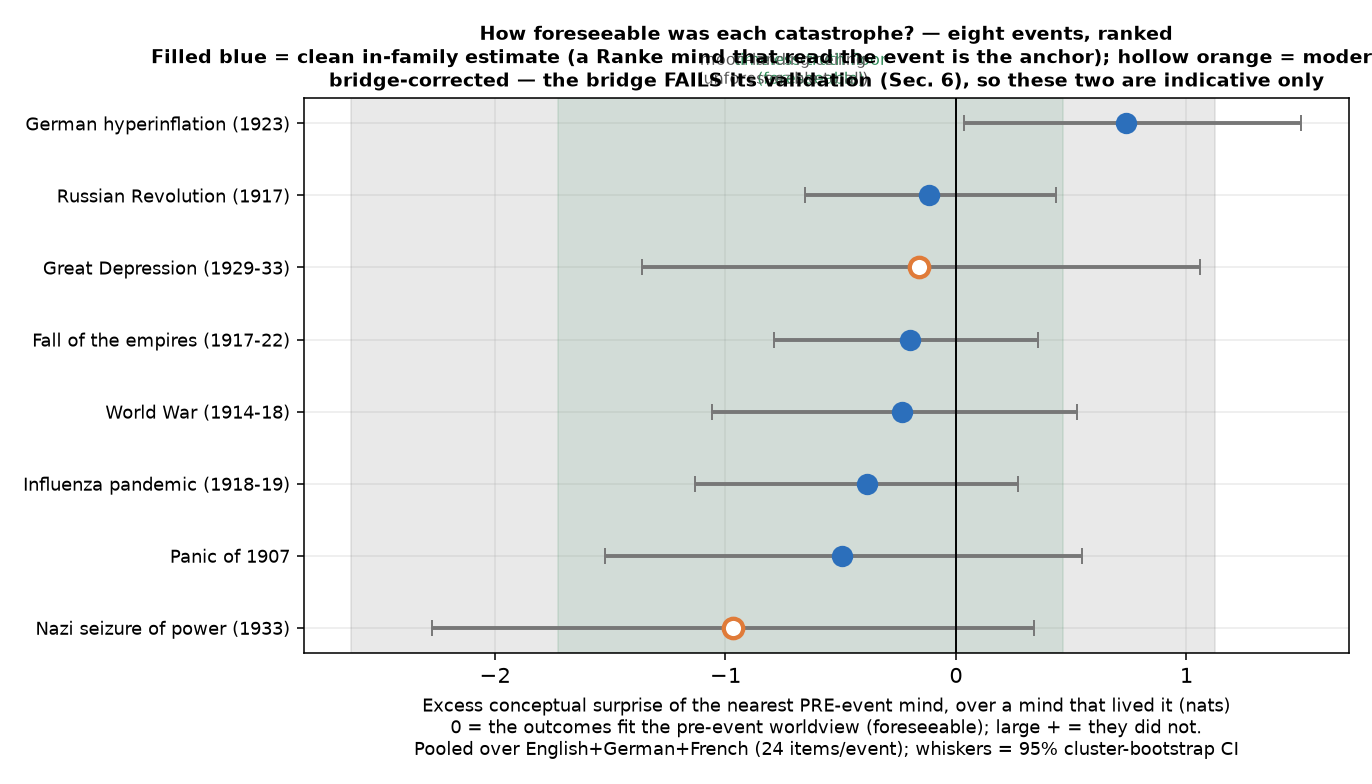
\includegraphics[width=.94\textwidth]{figP1_ranking.png}
\caption{\textbf{The foreseeability ranking.} The \emph{y-axis} lists the eight catastrophes; the
\emph{x-axis measures} the excess conceptual surprise of the nearest pre-event mind over a mind that lived
through the event (nats), pooled over English, German, and French (24 items per event); whiskers are 95\%
cluster-bootstrap confidence intervals. Zero means the outcomes fit the pre-event worldview --- foreseeable;
the green band is the timeless-truth floor, the grey band the moon-landing ceiling. Filled blue markers are
clean in-family estimates; hollow orange markers (Depression, Nazi seizure) are modern-anchored and
bridge-corrected, and the bridge fails its validation (Section~\ref{sec:bridge}), so they are indicative
only. \emph{Take-away:} panic, war, imperial collapse, revolution, and pandemic were all thinkable in
advance; the one in-family event that rises above the floor is the hyperinflation.}
\label{fig:ranking}
\end{figure}

\begin{table}[t]\centering\small
\begin{tabular}{lccrr}
\toprule
Event & Pre mind & Anchor & $\Delta_{\text{conc}}$ (pooled) & 95\% CI \\
\midrule
Nazi seizure of power (1933) & 1929 & modern (bridged) & $-0.97$ & $[-2.27,\,+0.34]$ \\
Panic of 1907 & 1900 & 1913 (in-family) & $-0.49$ & $[-1.52,\,+0.55]$ \\
Influenza pandemic (1918-19) & 1913 & 1929 (in-family) & $-0.39$ & $[-1.13,\,+0.27]$ \\
World War (1914-18) & 1913 & 1929 (in-family) & $-0.23$ & $[-1.06,\,+0.52]$ \\
Fall of the empires (1917-22) & 1913 & 1929 (in-family) & $-0.20$ & $[-0.79,\,+0.35]$ \\
Great Depression (1929-33) & 1929 & modern (bridged) & $-0.16$ & $[-1.36,\,+1.06]$ \\
Russian Revolution (1917) & 1913 & 1929 (in-family) & $-0.12$ & $[-0.66,\,+0.43]$ \\
German hyperinflation (1923) & 1913 & 1929 (in-family) & $+0.74$ & $[+0.04,\,+1.50]$ \\
\bottomrule
\end{tabular}
\caption{\textbf{The panel, ranked by pooled $\Delta_{\text{conc}}$ at the nearest pre-event mind.} An
in-family anchor means a Ranke model that read the event; ``modern (bridged)'' rows are indicative only
(Section~\ref{sec:bridge}). Pooled over three languages, 12 items per event per language; 95\%
cluster-bootstrap CIs.}
\label{tab:ranking}
\end{table}

\begin{table}[t]\centering\small
\begin{tabular}{lrrr}
\toprule
Event & English & German & French \\
\midrule
Nazi seizure of power (1933) & $+0.25$ & $-2.52$ & $-0.63$ \\
Panic of 1907 & $+0.15$ & $-0.82$ & $-0.81$ \\
Influenza pandemic (1918-19) & $-0.64$ & $+0.04$ & $-0.55$ \\
World War (1914-18) & $-0.77$ & $-0.45$ & $+0.53$ \\
Fall of the empires (1917-22) & $-0.58$ & $-0.03$ & $+0.01$ \\
Great Depression (1929-33) & $+0.55$ & $-1.67$ & $+0.64$ \\
Russian Revolution (1917) & $-0.69$ & $+1.18$ & $-0.83$ \\
German hyperinflation (1923) & $-0.12$ & $+0.95$ & $+1.39$ \\
\midrule
Timeless-truth floor & $-0.92$ & $+0.16$ & $-1.43$ \\
Moon-landing ceiling & $+0.82$ & $-2.32$ & $-0.05$ \\
\bottomrule
\end{tabular}
\caption{\textbf{The same estimates, language by language} ($\Delta_{\text{conc}}$ at the nearest pre-event
mind, mean over 12 items). The floor row is the timeless-truth control on the identical estimator; the
ceiling row is the future-to-all control after bridging --- its erratic German value is part of the
bridge's failed validation (Section~\ref{sec:bridge}).}
\label{tab:bylang}
\end{table}

Three validation checks, all passed, anchor the reading. First, the \emph{Panic of 1907} was included as a
positive control: financial panics were a recurring genre (1873, 1893 --- \citealp{bagehot1873}), so the
measure should read it as foreseeable, and it does ($\Npanpanic$ nats, judged by the 1900 mind against the
1913 mind). Second, twenty-four items carried over verbatim from our earlier three-language battery
reproduce their previous scores exactly --- same items, same models, same numbers --- so no part of tonight's
pipeline moved the goalposts. Third, the future-to-all controls read $\approx 0$ \emph{in-family} (the 1913
and 1929 minds are equally ignorant of the moon), as they must.

The substantive result is then the flatness of the ranking. The World War ($\Npanwwi$), the fall of the
empires ($\Npanemp$), the Russian Revolution ($\Npanrev$), the influenza pandemic ($\Npanflu$): each pooled
estimate sits within a nat of zero, each confidence interval straddles it, in English, German, and French
alike (Table~\ref{tab:bylang}). The written record of 1913 already contained the long war
\citep{bloch1899}, the brittle thrones, the revolution rehearsed in 1905, even the world-circling
pestilence --- pandemics, too, were a genre, and the 1889--92 influenza was in every newspaper the models
read. History's ``bolts from the blue'' were, to the minds that preceded them, weather.

\subsection{The exception: the death of money}\label{sec:infl}

One in-family event rises above the floor: the hyperinflation, at $\Npaninfl$ nats pooled --- the only
event whose confidence interval clears zero. The honest fine print: the signal is carried by French
($\NpaninflFR$, permutation $p=\NpaninflPFR$ against the French floor, the only event$\times$language cell
to survive the false-discovery correction) and by German ($\NpaninflDE$), while \emph{English reads the
death of money as foreseeable} ($\NpaninflEN$). No single item drives the result (the largest
leave-one-out shift is $0.46$ nats).

The asymmetry is historically legible, though we offer it as conjecture, not finding. The English-language
record of 1913 was saturated with monetary catastrophe as an \emph{argument}: the assignats, the
greenbacks, the free-silver wars, Jevons and the quantity theorists --- money-printing ruin was a standard
polemical trope. A French reader of 1913 lived instead inside the franc germinal, unchanged since 1803;
five generations of perfect monetary stability. What a worldview finds thinkable, our measure suggests, is
what its library kept arguing about \citep{keynes1923}.

\section{Pointing at the right catastrophe}\label{sec:selection}

That the true outcomes fit the pre-event worldview does not mean contemporaries would have \emph{picked}
them. For each event we therefore posed six matched duels: the outcome that happened against an equally
dramatic counterfactual that did not. A mind with real foresight prefers the truth; a measure that merely
rewards drama is indifferent; a mind in the grip of a wrong theory prefers the counterfactual.

\begin{figure}[t]\centering
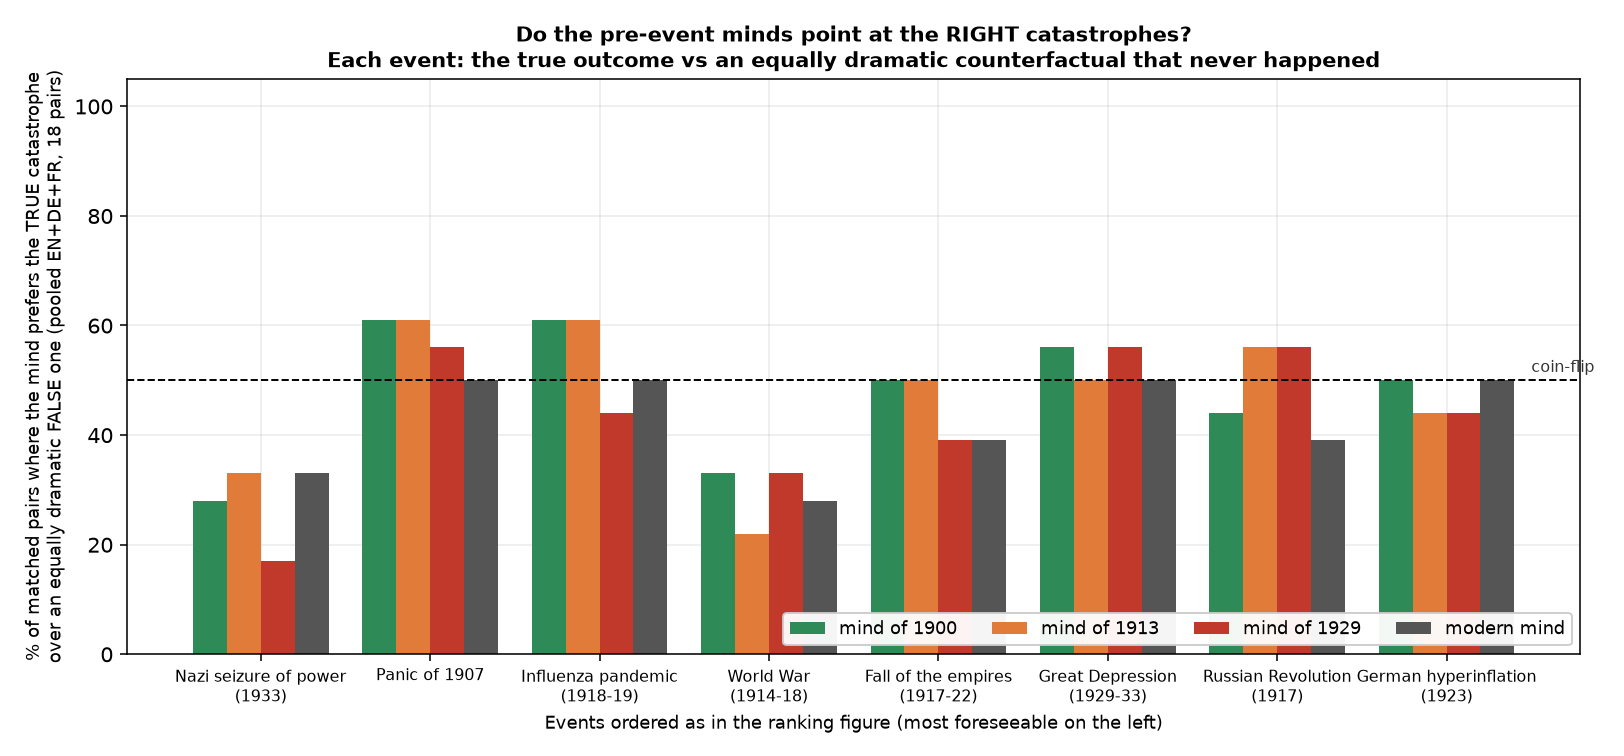
\includegraphics[width=.97\textwidth]{figP3_truefalse.png}
\caption{\textbf{Do the minds point at the right catastrophes?} The \emph{x-axis} lists the events, ordered
as in the ranking; the \emph{y-axis measures} the share of matched true/false pairs in which each mind
prefers the TRUE catastrophe (calibrated, pooled over three languages, 18 pairs per event); the dashed line
is a coin flip. Bars are the minds of 1900, 1913, 1929, and the modern mind. \emph{Take-away:} the
pre-event minds beat the coin where catastrophe was a recurring genre (the panic), sit at the coin for most
events, and fall \emph{below} it for the Nazi seizure --- they prefer the paths history did not take.}
\label{fig:tf}
\end{figure}

\begin{table}[t]\centering\small
\begin{tabular}{lrrrr}
\toprule
Event & mind of 1900 & 1913 & 1929 & modern \\
\midrule
Nazi seizure of power (1933) & 28\% & 33\% & 17\% & 33\% \\
Panic of 1907 & 61\% & 61\% & 56\% & 50\% \\
Influenza pandemic (1918-19) & 61\% & 61\% & 44\% & 50\% \\
World War (1914-18) & 33\% & 22\% & 33\% & 28\% \\
Fall of the empires (1917-22) & 50\% & 50\% & 39\% & 39\% \\
Great Depression (1929-33) & 56\% & 50\% & 56\% & 50\% \\
Russian Revolution (1917) & 44\% & 56\% & 56\% & 39\% \\
German hyperinflation (1923) & 50\% & 44\% & 44\% & 50\% \\
\bottomrule
\end{tabular}
\caption{\textbf{True-versus-false duels: share of pairs won by the truth, by mind.} Pooled over languages.
Pairs whose neutral frame retains the event identity have little discriminating power by construction
(they calibrate away the event itself); the informative rows are those whose false twin redirects the
catastrophe --- the panic, the pandemic, and above all the Nazi seizure.}
\label{tab:tf}
\end{table}

Three cells carry the story (Table~\ref{tab:tf}). The \emph{panic} duels reward the 1900 mind
($\Ntfpanicpre\%$): it knows the trust companies fall first ($\NtfPanicTrusts$ nats), knows the crash will
be severe ($\NtfPanicSevere$) --- panics were its native genre. The \emph{pandemic} duels split precisely
along the line of what the age could and could not think: the 1913 mind prefers ``a form of the familiar
influenza'' to ``the cholera come again'' ($\NtfFluFormPre$ nats) and places the pestilence in the last
year of the war ($\NtfFluWaryearPre$); but it bets the disease will spare the young ($\NtfFluYoungPre$) and
that science will find a serum in time ($\NtfFluSerumPre$). Form and timing: thinkable. The inverted
mortality curve and the helplessness of medicine: not.

And the \emph{Nazi seizure} inverts the coin ($\Ntfnazipre\%$ at the 1929 mind, mean margin
$\Ntfnazimargin$ nats). Branch by branch, the 1929 mind bets against the path history took: against lawful
appointment and for the armed march ($\NtfNaziLawful$); against the corporal and for the generals restoring
the Kaiser ($\NtfNaziCorporal$); against the aged president appointing the man he despised
($\NtfNaziPresident$); against cheering crowds and for civil war ($\NtfNaziCheering$). This is the
``confidently wrong'' signature our earlier English work found in ``home by Christmas'' --- now measured on
the death of a republic. The republic's actual death-path was the one branch its contemporaries had
discounted.

Free generation says the same thing in the models' own words. Prompted ``If Russia is beaten in a great
war, the Tsar will\dots'', the 1913 mind volunteers deposition in $\NprodRevTsarTh$ of its completions
(``be deposed and his son made Emperor''). Prompted for the next world-sweeping pestilence, it volunteers
influenza in $\NprodFluFormTh$ --- every mind names cholera, the last century's killer. Prompted with a
state paying its way by the printing press, it volunteers monetary death in $\NprodInflMarkTh$ of
completions --- gold-standard confidence to the end. And asked \emph{who} will rule Germany if the republic
fails, the 1929 mind names the corporal in $\NprodNaziWhoTN$ of completions; its greedy answer is ``not yet
in sight.'' In January 1933 that answer was four years stale.

\section{A correction: cross-family anchors carry a two-nat offset}\label{sec:bridge}

Our earlier three-language analysis anchored the Depression on the modern model and read its large excess
strain --- $\NxlDepXSEN$/$\NxlDepXSDE$/$\NxlDepXSFR$ nats at the 1929 mind in English/German/French --- as
unforeseeability in every language. The panel was designed to test that anchor, and the test failed the
anchor, not the event.

The instrument is simple: five panel events are \emph{in the 1929 model's corpus}. Whatever excess the 1929
mind shows against the modern mind on outcomes it has \emph{read} cannot be foresight failure; it is the
cross-family scale offset. Measured across those five events, the offset is $\NpanoffsetEN$ nats in
English, $\NpanoffsetDE$ in German, $\NpanoffsetFR$ in French. It is nearly as large as the excesses we had
been interpreting: the 1929 mind reads the World War --- which it lived through --- at
$\NwwiXSatTNEN$/$\NwwiXSatTNDE$/$\NwwiXSatTNFR$ nats against the modern anchor. Two nats of what we had
called unforeseeability is simply what \emph{any} Ranke mind scores against a modern model, event or no
event.

The pre-registered bridge --- subtract the offset, then require that the future-to-all controls still read
as unforeseeable --- fails its own validation: after bridging, the moon landing reads $\NtripCrawEN$ nats in
English but $\NtripCrawDE$ in German and $\NtripCrawFR$ in French (raw, at the 1913 mind). The German
failure traces to two control items whose archaic phrasing the modern model itself finds strained --- a
reminder that cross-family comparisons confound content with register, which is precisely why the in-family
estimator is the one this paper trusts.

Consequently: (i) our earlier three-language Depression claim is \textbf{withdrawn} --- it was mostly
offset; (ii) the bridged panel readings for the Depression ($\Npandep$) and the Nazi seizure ($\Npannazi$)
are reported hollow in Figure~\ref{fig:ranking} and carry no weight in our conclusions; (iii) what remains
of the Depression's exceptionalism is the one offset-free contrast from our registered English bank --- at
the same 1929 mind, Depression items exceed World-War items by $\NcontrastDiff$ nats (95\% CI
$\NcontrastCI$, $p=\NcontrastP$), a within-model difference no scale offset can produce --- corroborated on
real prose (Keynes and Angell, Hoover and Roosevelt: Depression DiD $\NtextDepDiDTN$ nats/char, CI
$\NtextDepCiTN$, against a World-War control of $\NtextWWIdidTh$). The panel's own within-1929 contrast,
built from different items, reads $\approx 0$. Two banks, two answers: the Depression's unforeseeability is
\emph{item-set dependent}, and we say so. A Ranke model trained to 1938 would anchor it in-family and
settle the question; until then, 1929 is open.

\section{The contamination gate}\label{sec:gate}

A low $\Delta_{\text{conc}}$ is foresight only if the pre-event model does not secretly know the outcome.
For every event, in every language, six post-event fact probes ran under the event's pre-event mind ---
four-way calibrated forced choice, chance $=25\%$ --- and, as a probe-validity ceiling, under the event's
anchor.

\begin{table}[t]\centering\small
\begin{tabular}{lcllll}
\toprule
Event & Pre mind & Gate (pre) & correct & Ceiling & correct \\
\midrule
Panic of 1907 & 1900 & GREEN & 3/15 & OK & 10/15 \\
World War (1914-18) & 1913 & GREEN & 7/15 & OK & 14/15 \\
Fall of the empires (1917-22) & 1913 & GREEN & 7/15 & OK & 8/15 \\
Russian Revolution (1917) & 1913 & AMBER$^{\dagger}$ & 9/18 & OK & 10/18 \\
Influenza pandemic (1918-19) & 1913 & GREEN & 6/18 & OK & 9/18 \\
German hyperinflation (1923) & 1913 & GREEN & 5/18 & OK & 11/18 \\
Great Depression (1929-33) & 1929 & GREEN & 5/15 & OK & 12/15 \\
Nazi seizure of power (1933) & 1929 & GREEN & 5/18 & WEAK-PROBES & 8/18 \\
\bottomrule
\end{tabular}
\caption{\textbf{The gate, event by event.} GREEN = accuracy consistent with chance (binomial test): the
pre-event mind does not know the post-event facts, so its low conceptual surprise is foresight, not
leakage. The ceiling column shows the same probes under the hindsight anchor --- high accuracy there
validates the probes themselves. Items with pre-registered period-prior caveats (Morgan, Versailles,
Franz Ferdinand, Roosevelt) are excluded from verdicts and reported separately.
$^{\dagger}$The revolution's AMBER is driven by a single geography item (the peace ``at Brest-Litovsk,''
answered 3/3 while Lenin, the party, and the month sit at the floor) --- the signature of a place-name
prior, not event knowledge; excluding it post hoc gives $\Ngaterevposthoc$ ($p=\NgaterevposthocP$), GREEN.
The registered verdict stands, and the caveat travels with the revolution's foresight reading.}
\label{tab:gates}
\end{table}

Seven of eight events gate GREEN (Table~\ref{tab:gates}). The minds that read the panic, the pandemic, and
the hyperinflation as thinkable cannot date them, name them, or place them: the 1913 mind does not know the
pandemic will be called Spanish, the 1900 mind cannot name the Knickerbocker, the 1929 mind puts the
slump's trough anywhere but 1932. The one AMBER --- the revolution --- dissolves under item-level
inspection into a Brest-Litovsk geography prior (see the table note), and the one weak ceiling (the Nazi
probes under the modern 3B model) means that gate is less informative, not that it failed. The tripwire
held everywhere in-family: no pre-1930 model finds the moon landing easy against the 1929 anchor.

\section{Inside the English bank: mechanics and corroboration}\label{sec:english}

The panel's conclusions inherit the machinery our registered English bank established; we summarize what
carries over. The World War's \emph{raw} excess surprise at the 1913 mind is large ($\NwwidSTh$ nats) but
almost entirely lexical: the same-tokenizer split assigns $\NwwiDlexTh$ to vocabulary and
$\NwwiDconcTh$ --- zero --- to the idea (Figure~\ref{fig:wwisplit}). ``Home by Christmas'' was a mood, not a
worldview: under length-matched forced choice the 1913 mind puts the probability mass on the long war, and
in free generation it volunteers ``for years'' in every sampled completion, while never volunteering the
war's scale in lives. Recognition exceeds production throughout --- the sterner test agrees with the duels
of Section~\ref{sec:selection}: thinkable, rarely chosen.

\begin{figure}[t]\centering
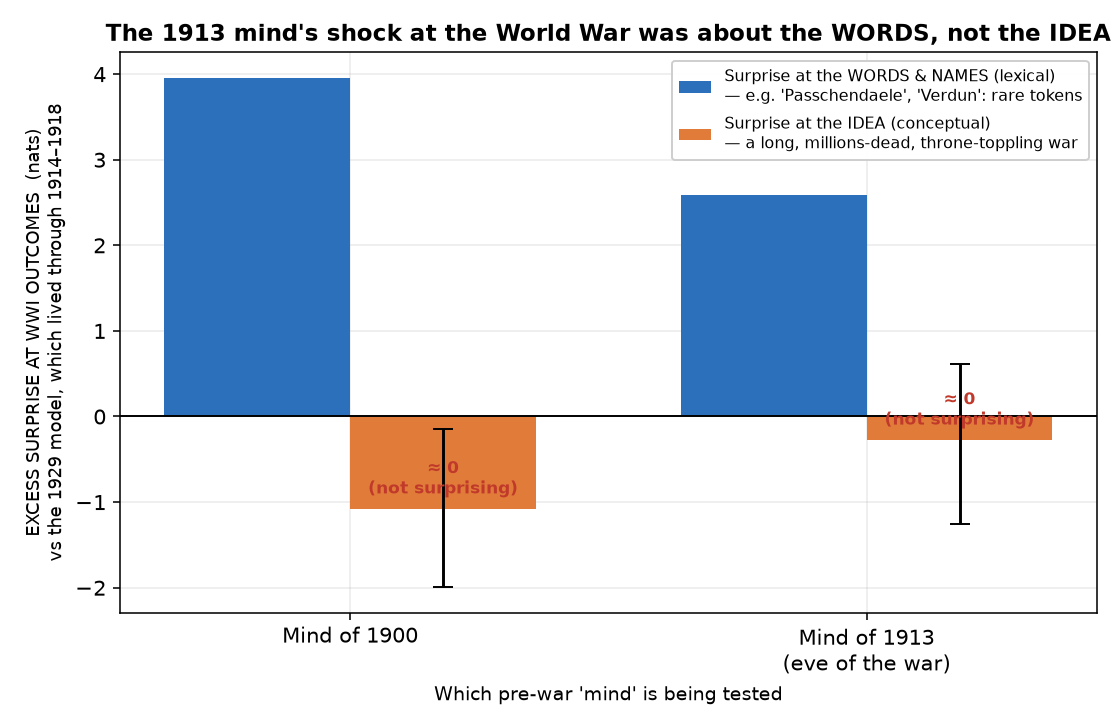
\includegraphics[width=.8\textwidth]{fig2_wwi_split.png}
\caption{\textbf{The war's surprise was words, not ideas.} The \emph{x-axis} shows the pre-war mind (1900
or 1913); the \emph{y-axis measures} its excess surprise at the war's outcomes relative to the 1929 mind
(nats), split into surprise at new \emph{words and names} (blue) and surprise at the \emph{idea} (orange);
whiskers are 95\% CIs. \emph{Take-away:} strip the unfamiliar vocabulary and nothing is left --- the war's
character was not a new idea in 1913.}
\label{fig:wwisplit}
\end{figure}

On genuine period prose the same pattern holds (Arm B): measuring per-character surprise --- the
tokenizer-independent channel --- with the author held fixed across the shock, the World War passes its own
control ($\NtextWWIdidTh$ nats/char, CI $\NtextWWIciTh$), while Depression-era prose stays foreign to every
pre-1930 mind ($\NtextDepDiDTN$ at the 1929 mind, CI $\NtextDepCiTN$). That real-text contrast is
offset-free by construction and remains the strongest single piece of evidence that 1929 differed in kind
--- standing, per Section~\ref{sec:bridge}, as an open question the panel could not close.

\section{The worldview itself: Zweig, retested}\label{sec:zweig}

\citet{zweig1942} catalogued four illusions of the pre-1914 mind: irresistible progress, the unthinkability
of war, the confinement of women, the veneration of age. We rebuilt the battery at full strength --- five
calibrated belief-versus-skeptic items per theme, the women's items now purely normative --- and the
enlarged battery \emph{narrows} our earlier claims (Figure~\ref{fig:zweig}).

The unthinkability of war remains robustly \emph{French} ($\NzwiiiwarFR$ nats at 1913, rejected by the
modern mind at $\NzwiiiwarModFR$) and robustly absent in English --- the 1913 English mind \emph{expects}
war ($\NzwiiiwarEN$) --- but German, positive in the three-item battery, turns ambiguous at five items
($\NzwiiiwarDE$): Zweig's ``as impossible as witches and ghosts'' survives, in our measurement, principally
in his neighbours' French. Faith in progress stays positive at 1913 in all three languages
($\NzwiiiprogressEN$/$\NzwiiiprogressDE$/$\NzwiiiprogressFR$) but the time-locked-minus-modern gap shrinks
with the battery. The confinement of women and the cult of age do not register as time-locked beliefs at
any battery size we tried; five items, normative-only, French re-phrased --- still nothing. We report them
as the measure's limits, not as findings, and we flag the battery-size sensitivity itself as a caution
attaching to all worldview (as opposed to event) probes.

\begin{figure}[t]\centering
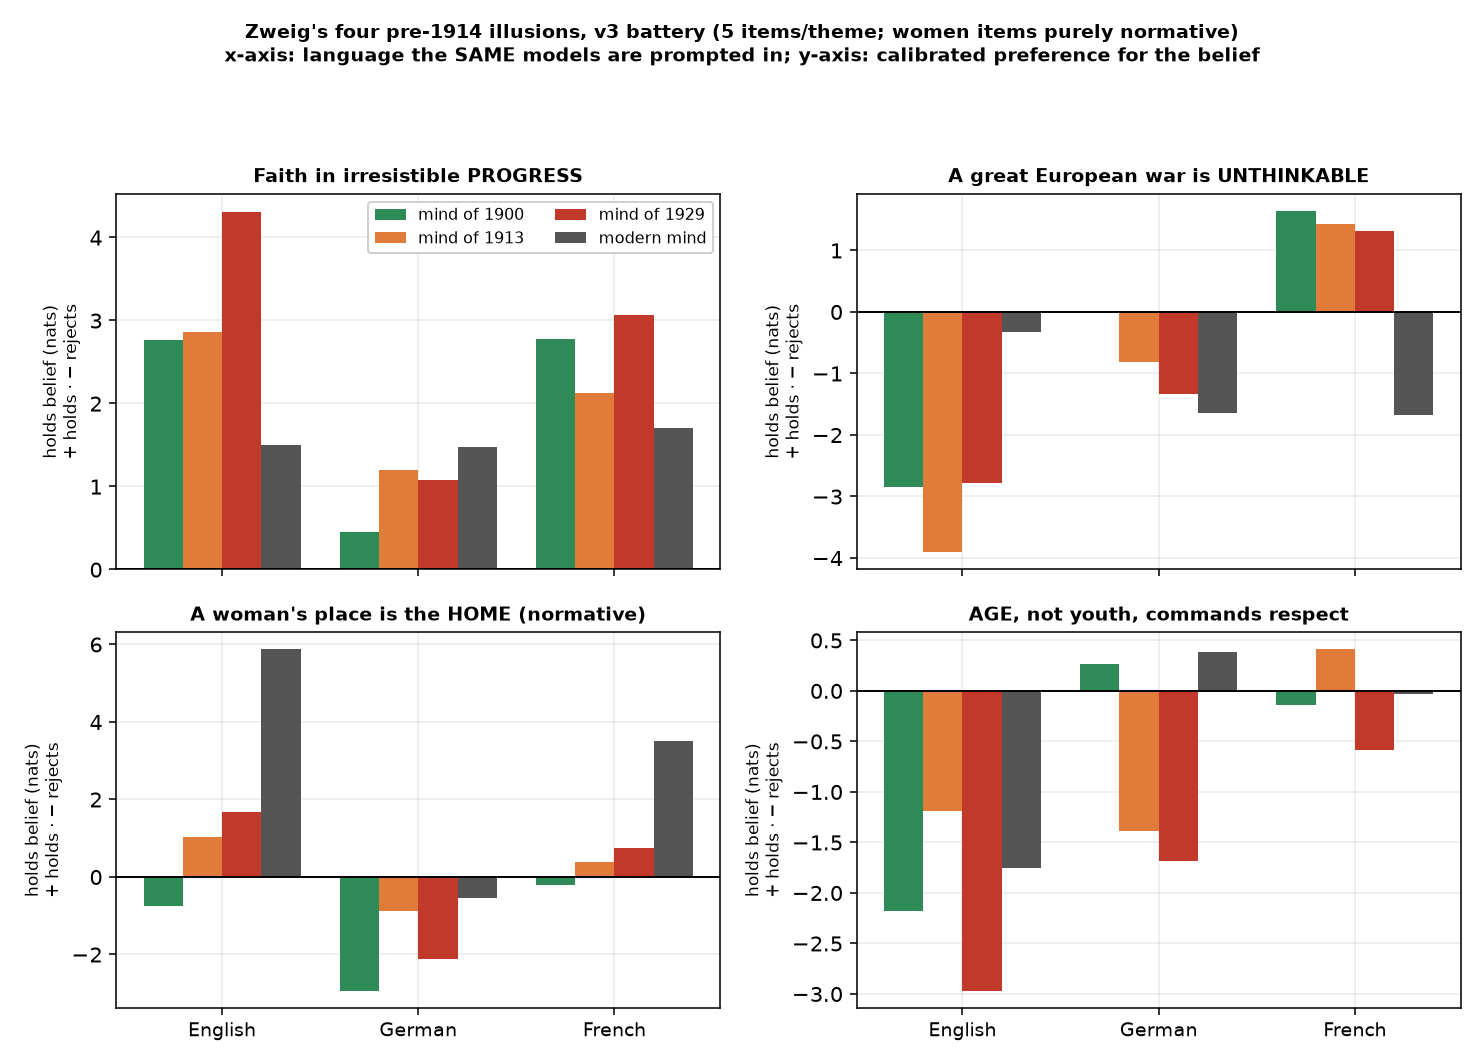
\includegraphics[width=.95\textwidth]{figP4_zweig.png}
\caption{\textbf{Zweig's four illusions at full battery strength.} Each panel is one theme; the
\emph{x-axis} is the language the same models are prompted in; the \emph{y-axis measures} the calibrated
preference for the pre-1914 belief over its opposite (nats; $+$ holds the illusion). Bars are the minds of
1900, 1913, 1929, and the modern mind. \emph{Take-away:} war-unthinkability is French (and rejected by the
modern mind); the English mind expects war; progress is held everywhere but more weakly than smaller
batteries suggested; women and youth do not register --- honest holdouts.}
\label{fig:zweig}
\end{figure}

\section{Limitations}\label{sec:limits}

The models are 4-billion-parameter readers of incomplete corpora; a null ``no inkling detected'' bounds
what the \emph{written record} contained, not what any individual believed, and the Bloch minority that
foresaw attrition reminds us the record was not unanimous. The bridge failure means we currently have
\emph{no} trustworthy cross-family estimator: everything in this paper that carries weight is in-family,
and the two post-1929 events therefore wait on a later time-locked model. The true/false duels lose power
wherever the neutral frame retains the event identity --- a design cost of calibration we document rather
than hide. The hyperinflation exception is language-dependent (French-led, English-null) and, while it
survives FDR and leave-one-out checks, twelve items per language is a modest base for the panel's one
positive claim. Worldview probes are battery-sensitive (Section~\ref{sec:zweig}). And all results are
conditional on corpus composition --- a 1913 model has read disproportionately what was printed and kept,
which is itself a period artifact.

\section{Conclusion}

Foreseeability is measurable, and for the early twentieth century the measurement reverses the cliché. The
catastrophes were not bolts from a clear sky: panic, world war, the fall of the empires, revolution, and
pandemic all fit the pre-event worldview as comfortably as the turning of the seasons, in English, German,
and French alike --- and the minds that found them thinkable demonstrably did not know the facts
(Section~\ref{sec:gate}). The scarce thing was not imagination but \emph{selection}: the same 1929 mind
that could think the republic's death bet, branch by branch, on every path except the lawful one it took;
the same 1913 mind that could think a world-circling influenza expected cholera, a serum, and the sparing
of the young. Where the record had argued a catastrophe for decades --- panics in English, monetary ruin in
the quantity-theory tradition --- the minds even \emph{point} at the truth; where it had not, they point
confidently elsewhere. That is a sharper indictment of ex-ante forecasting than unforeseeability would have
been: the futures were on the shelf; contemporaries picked the wrong ones. And one methodological result we
did not want but must keep: cross-family model comparisons carry a two-nat scale offset that mimics
unforeseeability --- it manufactured our own earlier Depression claim, which we withdraw. The Depression
question is open, and openable: train the 1938 model, and the same machinery that ranked 1907--1923 will
close it.

\begin{thebibliography}{99}
\bibitem[Angell(1910)]{angell1910} Angell, Norman. 1910. \emph{The Great Illusion: A Study of the Relation of
Military Power to National Advantage}. London: William Heinemann.
\bibitem[Bagehot(1873)]{bagehot1873} Bagehot, Walter. 1873. \emph{Lombard Street: A Description of the Money
Market}. London: Henry S. King.
\bibitem[Barro(2006)]{barro2006} Barro, Robert J. 2006. ``Rare Disasters and Asset Markets in the Twentieth
Century.'' \emph{Quarterly Journal of Economics} 121(3): 823--866.
\bibitem[Bloch(1899)]{bloch1899} Bloch, Ivan S. 1899. \emph{Is War Now Impossible?} London: Grant Richards.
\bibitem[Fisher(1930)]{fisher1930} Fisher, Irving. 1930. \emph{The Stock Market Crash---and After}. New York:
Macmillan.
\bibitem[Hoover(1929)]{hoover1929} Hoover, Herbert. 1929. Inaugural Address, March 4, 1929.
\bibitem[Keynes(1919)]{keynes1919} Keynes, John Maynard. 1919. \emph{The Economic Consequences of the Peace}.
London: Macmillan.
\bibitem[Keynes(1923)]{keynes1923} Keynes, John Maynard. 1923. \emph{A Tract on Monetary Reform}. London:
Macmillan.
\bibitem[Kuran(1991)]{kuran1991} Kuran, Timur. 1991. ``Now Out of Never: The Element of Surprise in the East
European Revolution of 1989.'' \emph{World Politics} 44(1): 7--48.
\bibitem[Rietz(1988)]{rietz1988} Rietz, Thomas A. 1988. ``The Equity Risk Premium: A Solution.''
\emph{Journal of Monetary Economics} 22(1): 117--131.
\bibitem[Roosevelt(1933)]{roosevelt1933} Roosevelt, Franklin D. 1933. First Inaugural Address, March 4, 1933.
\bibitem[Zweig(1942)]{zweig1942} Zweig, Stefan. 1942. \emph{The World of Yesterday} (\emph{Die Welt von
Gestern}). Stockholm: Bermann-Fischer.
\end{thebibliography}

\end{document}
